\documentclass{standalone}
\usepackage{tikz}
\usetikzlibrary{arrows,decorations.markings,calc,positioning}

% from http://tex.stackexchange.com/a/163695
\tikzset{
   set arrow inside/.code={\pgfqkeys{/tikz/arrow inside}{#1}},
   set arrow inside={end/.initial=>, opt/.initial=},
   /pgf/decoration/Mark/.style={
      mark/.expanded=at position #1 with
      {
         \noexpand\arrow[\pgfkeysvalueof{/tikz/arrow inside/opt}]{\pgfkeysvalueof{/tikz/arrow inside/end}}
      }
   },
   arrow inside/.style 2 args={
      set arrow inside={#1},
      postaction={
         decorate,decoration={
            markings,Mark/.list={#2}
         }
      }
   },
}

\ifdefined\argempty
\fi

\ifdefined\argdrawaxes
   \def\drawaxes{}
\fi

\ifdefined\argdrawa
   \def\drawaxes{}
   \def\drawa{}
\fi

\ifdefined\argdrawab
   \def\drawaxes{}
   \def\drawa{}
   \def\drawb{}
\fi

\ifdefined\argdrawabxstar
   \def\drawaxes{}
   \def\drawa{}
   \def\drawb{}
   \def\drawxstar{}
\fi

\ifdefined\argdrawabxstarc
   \def\drawaxes{}
   \def\drawa{}
   \def\drawb{}
   \def\drawxstar{}
   \def\drawc{}
\fi

\ifdefined\argdrawabxstarcd
   \def\drawaxes{}
   \def\drawa{}
   \def\drawb{}
   \def\drawxstar{}
   \def\drawc{}
   \def\drawd{}
\fi

\ifdefined\argdrawabxstarcdutility
   \def\drawaxes{}
   \def\drawa{}
   \def\drawb{}
   \def\drawxstar{}
   \def\drawc{}
   \def\drawd{}
   \def\drawutility{}
\fi

\begin{document}
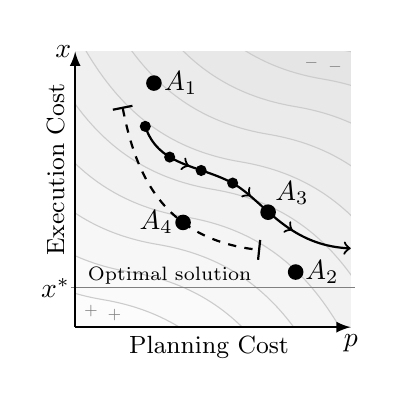
\begin{tikzpicture}

\draw[step=0.1,black!15,very thin,opacity=0.0] (-0.6,-0.6) grid (3.8,3.8);

% contours
\ifdefined\drawutility
\begin{scope}
   \clip (0,0) rectangle (3.5,3.5);
   \foreach \s in {10,...,1}
   {
      \begin{scope}[shift={($(0.35*\s,0.35*\s)$)}]
      
         \coordinate (parama) at (-2.0, 4.5);
         \coordinate (paramb) at (-3.0, 0.5);
         \coordinate (paramc) at ( 3.0,-0.5);
         \coordinate (paramd) at ( 2.0,-4.5);
      
         \draw[black!20,fill=black!\s]
         (-5.0,5.0) .. controls (parama) and (paramb) .. 
         (0.0, 0.0) .. controls (paramc) and (paramd) .. (5.0,-5.0)
          -- (-5.0,-5.0) -- cycle;
          
         %\node[circle,fill=blue,inner sep=0.1cm] at (parama) {};
         %\node[circle,fill=blue,inner sep=0.1cm] at (paramb) {};
         %\node[circle,fill=blue,inner sep=0.1cm] at (paramc) {};
         %\node[circle,fill=blue,inner sep=0.1cm] at (paramd) {};
         
      \end{scope}
   }
\end{scope}

\node[text=black!50] at (0.2,0.20) {\tiny $+$};
\node[text=black!50] at (0.5,0.15) {\tiny $+$};
\node[text=black!50] at (3.0,3.35) {\tiny $-$};
\node[text=black!50] at (3.3,3.30) {\tiny $-$};
\fi

\ifdefined\drawxstar
   \draw[black!50] (-0.05,0.5) -- (3.55,0.5); % optimal path
   \node at (1.2,0.65) {\scriptsize Optimal solution};
\fi

% simple point
\ifdefined\drawa
   \node[circle,fill=black,inner sep=0.07cm] (a1) at (1.0,3.1) {};
   \node[right=-0.1cm of a1] {$A_1$};
\fi

\ifdefined\drawb
   \node[circle,fill=black,inner sep=0.07cm] (a2) at (2.8,0.7) {};
   \node[circle,right=-0.20cm of a2] {$A_2$};
\fi

% anytime
\ifdefined\drawc
   \draw[black,thick,->,
      arrow inside={end=>,opt={black}}{0.25,0.53,0.75}]
      (0.89,2.55)
      .. controls (1.05,2.06) and (1.54,2.06) .. (1.96,1.85)
      .. controls (2.38,1.64) and (2.67,1.04) .. (3.50,1.0);
   \node[circle,fill=black,inner sep=0.05cm] at (0.89,2.55) {};
   \node[circle,fill=black,inner sep=0.05cm] at (1.2,2.16) {};
   \node[circle,fill=black,inner sep=0.05cm] at (1.6,1.99) {};
   \node[circle,fill=black,inner sep=0.05cm] at (2.0,1.83) {};
   \node[circle,fill=black,inner sep=0.07cm] (a4) at (2.45,1.46) {};
   \node[above right=-0.15cm of a4] {$A_3$};
\fi

% parameterized
\ifdefined\drawd
   \draw[black,thick,dashed,|-|]
      (0.6,2.8) .. controls (0.74,2.1) and (1.02,1.12) .. (2.35,0.98);
   \node[circle,fill=black,inner sep=0.07cm] (a3) at (1.37,1.33) {};
   \node[left=-0.1cm of a3] {$A_4$};
\fi

\draw[thick,-latex] (0,0) -- (3.5,0); % x axis
\draw[thick,-latex] (0,0) -- (0,3.5); % y axis

\ifdefined\drawaxes
   % labels
   \node at (1.7,-0.25) {\small Planning Cost};
   \node[rotate=90] at (-0.25,2) {\small Execution Cost};

   \node at (3.5,-0.2) {$p$};
   \node at (-0.15,3.5) {$x$};
\fi

\ifdefined\drawxstar
   \node at (-0.25,0.5) {$x^*$};
\fi

\end{tikzpicture}
\end{document}
